\documentclass[12pt,a4paper]{article}
\usepackage[czech]{babel}
\usepackage[T1]{fontenc}
\usepackage[utf8]{inputenc}

\usepackage{graphicx} % Required for including pictures
\graphicspath{{Pictures/}} % Specifies the directory where pictures are stored

\usepackage{hyperref} % URLs
\usepackage{syntax} % Grammar typesetting
\usepackage{minted} % Program highlighting

\begin{document}

%----------------------------------------------------------------------------------------
%	TITLE PAGE
%----------------------------------------------------------------------------------------

\begin{titlepage}

\newcommand{\HRule}{\rule{\linewidth}{0.5mm}} % Defines a new command for the horizontal lines, change thickness here

\center % Center everything on the page


\includegraphics[width=0.5\textwidth]{logo-fav.png}~\\[2cm] % Include a department/university logo - this will require the graphicx package

\textsc{\Large KIV/FJP --- Semestrální práce}\\[0cm]


\HRule \\[0.8cm]
\begin{center}
 \Huge \bfseries Překladač Rustu pro LLVM\\[0.4cm] % Title of your document
\end{center}
\HRule \\[0.5cm]

\vspace{\fill}

\begin{minipage}{0.4\textwidth}
\begin{flushleft} \large
\emph{Datum:} \\
\today\\[0.2cm] % Date, change the \today to a set date if you want to be precise


\emph{Autoři:}\\
Jiří \textsc{Láska}\\
Václav \textsc{Löffelmann}\\ 
Martin \textsc{Váňa}\\[0.2cm] % Our names



\end{flushleft}
\end{minipage}
~
\begin{minipage}{0.4\textwidth}
\begin{flushright} \large


\emph{Název týmu:} \\
Falsum $\bot$\\[0.2cm] % Date, change the \today to a set date if you want to be precise

\emph{Emaily:} \\
\href{mailto:goheeca@students.zcu.cz}{goheeca@students.zcu.cz}\\
\href{mailto:loffelmv@students.zcu.cz}{loffelmv@students.zcu.cz}\\
\href{mailto:vanam@students.zcu.cz}{vanam@students.zcu.cz}\\[0.2cm] % Date, change the \today to a set date if you want to be precise


\end{flushright}
\end{minipage}\\

\end{titlepage}


%----------------------------------------------------------------------------------------
%	TOC
%----------------------------------------------------------------------------------------
\thispagestyle{empty}

\tableofcontents


\newpage


\setcounter{page}{3}

%----------------------------------------------------------------------------------------
%	TASK
%----------------------------------------------------------------------------------------

\section{Zadání}

Cílem práce bude vytvoření překladače zvoleného jazyka. Je možné inspirovat se jazykem PL/0, vybrat si podmnožinu nějakého existujícího jazyka nebo si navrhnout jazyk zcela vlastní. Dále je také potřeba zvolit si pro jakou architekturu bude jazyk překládán (doporučeny jsou instrukce PL/0, ale je možné zvolit jakoukoliv instrukční sadu pro kterou budete mít interpret).\\

\noindent
Jazyk musí mít minimálně následující konstrukce:

\begin{itemize}
	\item definice celočíselných proměnných
    \item definice celočíselných konstant
    \item přiřazení
    \item základní aritmetiku a logiku (+, -, *, /, AND, OR, negace a závorky)
    \item cyklus (libovolný)
    \item jednoduchou podmínku (\texttt{if} bez \texttt{else})
    \item definice podprogramu (procedura, funkce, metoda) a jeho volání
\end{itemize}

\noindent
Překladač který bude umět tyto základní věci bude hodnocen deseti body. Další body je možné získat na základě rozšíření, každé je za 2 body:

\begin{itemize}
    \item další typ cyklu (\texttt{for}, \texttt{do .. while}, \texttt{while .. do}, \texttt{repeat .. unitl)}
    \item \texttt{else} větev
    \item příkaz \texttt{goto} (pozor na vzdálené skoky)
    \item datový typ \texttt{boolean} a logické operace s ním
    \item datový typ \texttt{real} (s celočíselnými instrukcemi)
    \item datový typ \texttt{ratio} (s celočíselnými instrukcemi)
    \item složený datový typ (\texttt{Record})
    \item pole
    \item příkazy pro vstup a výstup (\texttt{read}, \texttt{write} - potřebuje vhodné instrukce které bude možné využít)
    \item rozvětvená podmínka (\texttt{switch}, \texttt{case})
    \item násobné přiřazení (\texttt{a = b = c = d = 3;})
    \item podmíněné přiřazení / ternární operátor (\texttt{min = (a < b) ? a : b;})
    \item paralelní přiřazení (\texttt{\{a, b, c, d\} = \{1, 2, 3, 4\};})
    \item parametry předávané odkazem
    \item parametry předávané hodnotou
    \item návratová hodnota podprogramu
    \item ...
\end{itemize}

%----------------------------------------------------------------------------------------
%	ANALYSIS
%----------------------------------------------------------------------------------------

\section{Analýza}

\begin{figure}
\centering
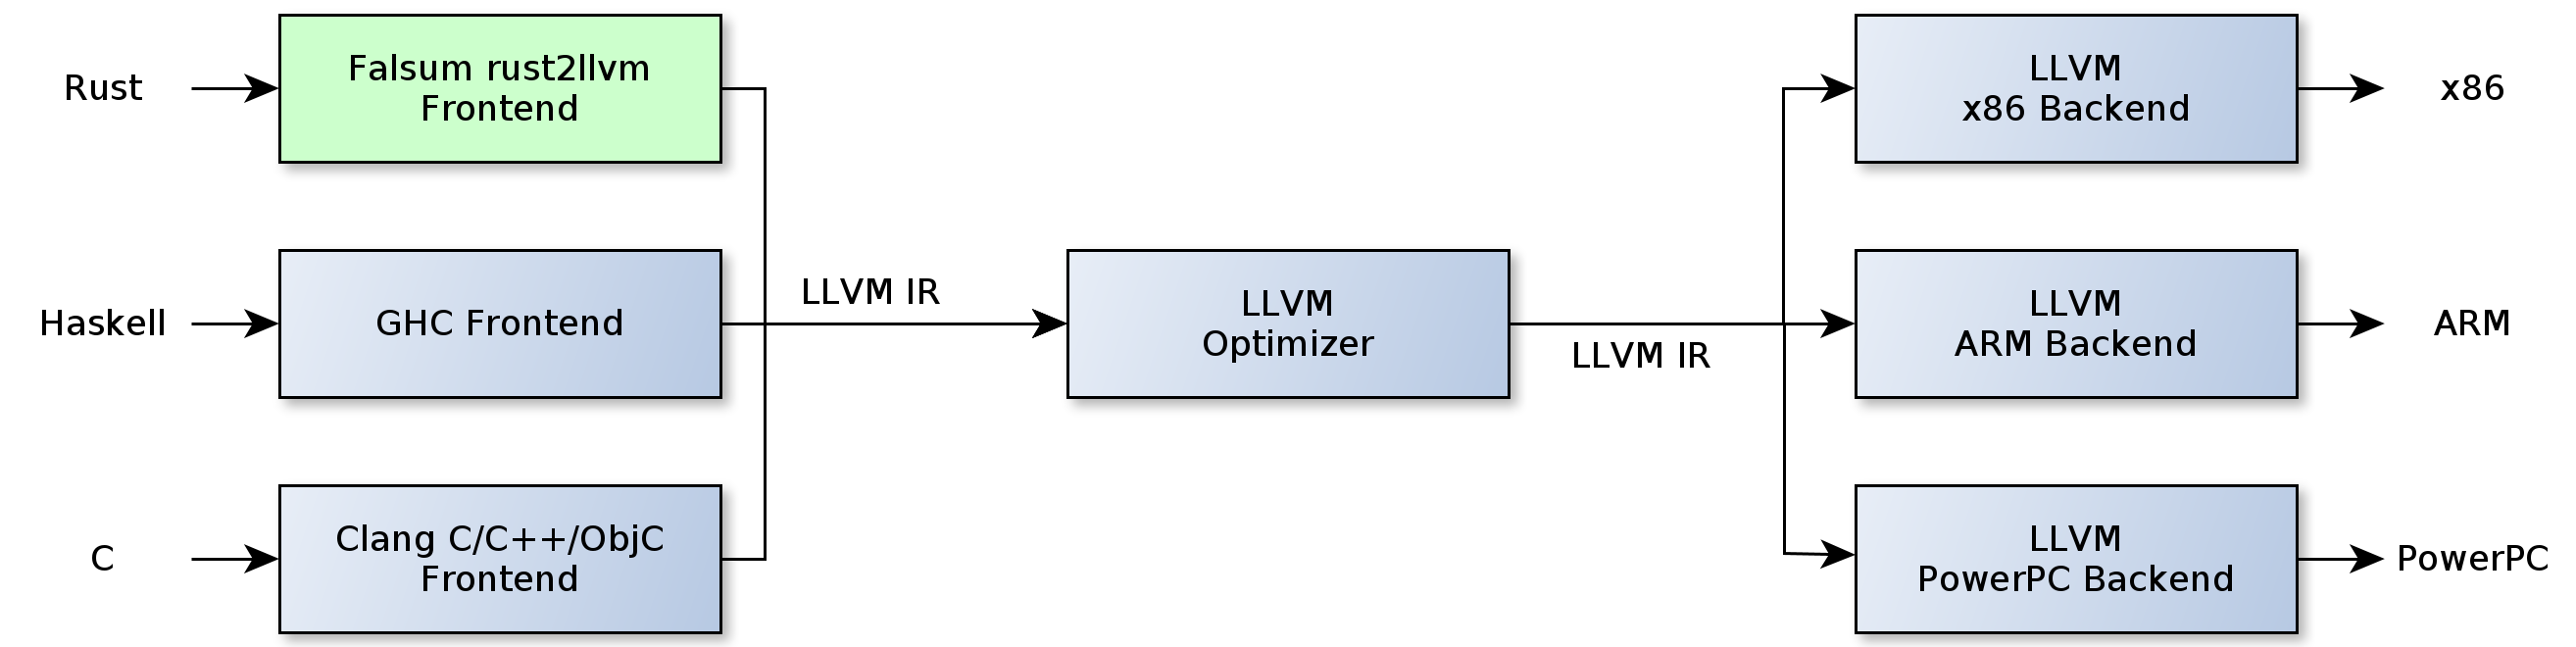
\includegraphics[width=1\textwidth]{compiler-schema.png}
\caption{Schéma překladače}
\label{img:compiler-schema}
\end{figure}

Jako zadání semestrální práce jsme si zvolili implementaci překladače podmnožiny jazyka Rust\footnote{\url{https://www.rust-lang.org/}} do mezikódu LLVM\footnote{\url{http://llvm.org/}}. 

Rust je moderní programovací jazyk, jenž si bere za cíl být srovnatelně rychlý jako C či C++ a zároveň bezpečný (ve smyslu zamezení programátorovi ve vytvoření chyb typických pro C/C++, typicky při správě paměti).

LLVM je projekt, který obsahující mnoho nástrojů usnadňující tvorbu překladačů. LLVM IR (\textit{Intermediate Representation}) je univerzální mezijazyk, který kompilátor LLVM přeloží do spustitelné binárky pro danou platformu.

Cílem práce je tedy tvorba vlastního frontendu viz obrázek~\ref{img:compiler-schema} pro LLVM (kaskádní překladač). Z edukativních účelů jsme programovali v jazyce Haskell.\\

Pozn.: Oficiální překladač Rustu je implementován přesně tímto způsobem, ale v frontend je napsaný jazyce C.

%----------------------------------------------------------------------------------------
%	GRAMMAR
%----------------------------------------------------------------------------------------

\section{Gramatika jazyka}

\setlength{\grammarparsep}{20pt plus 1pt minus 1pt} % increase separation between rules
\setlength{\grammarindent}{12em} % increase separation between LHS/RHS 

TODO doplnit

\begin{grammar}

<statement> ::= <ident> `=' <expr> 
\alt `for' <ident> `=' <expr> `to' <expr> `do' <statement> 
\alt `{' <stat-list> `}' 
\alt <empty> 

<stat-list> ::= <statement> `;' <stat-list> | <statement> 

\end{grammar}

%----------------------------------------------------------------------------------------
%	LANGUAGE SUBSET
%----------------------------------------------------------------------------------------

\section{Podporované jazykové konstrukce}

\subsection{Základní}

\subsubsection*{Lokální proměnné}

\begin{minted}[autogobble]{rust}
let a: i32;
\end{minted}

\subsubsection*{Globální proměnné}

\begin{minted}[autogobble]{rust}
static M: i32;
\end{minted}

\subsubsection*{Globální konstanty}

\begin{minted}[autogobble]{rust}
const ANSWER: i32;
\end{minted}

\subsubsection*{Přiřazení}

\begin{minted}[autogobble]{rust}
a = 5;
\end{minted}

\subsubsection*{Základní aritmetika}

\begin{minted}[autogobble]{rust}
a = b + c;
a = b - c;
a = b * c;
a = b / c;
a = b & c;
a = b | c;
a = b;
a = (a + b) * c;
\end{minted}

\subsubsection*{Nekonečný cyklus}

\begin{minted}[autogobble]{rust}
loop {...}
\end{minted}

\subsubsection*{Jednoduchá podmínka}

\begin{minted}[autogobble]{rust}
if a == 1 {...}
\end{minted}

\subsubsection*{Definice funkce}

\begin{minted}[autogobble]{rust}
fn foo() {...}
\end{minted}

\subsection{Rozšíření}

\subsubsection*{Cyklus while}

\begin{minted}[autogobble]{rust}
while a > b {...}
\end{minted}

\subsubsection*{else větev}

\begin{minted}[autogobble]{rust}
if a == 1 {...} else {...}
\end{minted}

\subsubsection*{Vícenásobná podmínka}

\begin{minted}[autogobble]{rust}
if a == 1 {...} else if a == 2 {...} else {...}
\end{minted}

\subsubsection*{Datový typ boolean a operace s ním}

\begin{minted}[autogobble]{rust}
let x: bool = true;

a = b & c;
a = b | c;
a = b ^ c;
a = b << c;
a = b >> c;
a = !b;
\end{minted}

\subsubsection*{Datový typ real}

\begin{minted}[autogobble]{rust}
let x: f32;
\end{minted}

\subsubsection*{printf}

\begin{minted}[autogobble]{rust}
printf("a = %d\n", a);
\end{minted}

\subsubsection*{Násobné přiřazení}

\begin{minted}[autogobble]{rust}
a = b = c = d = 3
\end{minted}

\subsubsection*{Podmíněné přiřazení}

\begin{minted}[autogobble]{rust}
a = if a == 1 { b } else { c };
\end{minted}

\subsubsection*{Parametry předávané hodnotou}

\begin{minted}[autogobble]{rust}
fn foo(a: i32, b: bool) {...}

foo(1, true);
\end{minted}

\subsubsection*{Definice funkce s návratovou hodnotou}

\begin{minted}[autogobble]{rust}
fn bar() : i32 {
    ...
    foo();
    ...
    retun 0;
}
\end{minted}

%----------------------------------------------------------------------------------------
%	IMPLEMENTATION
%----------------------------------------------------------------------------------------

\section{Implementace}

Vlastní překlad je rozdělen do tří částí -- lexeru, parseru a generátoru kódu. Vstupem je zdrojový kód v Rustu a výstupem je mezijazyk LLVM IR, který následně přeložíme pomocí Clangu do spustitelné binárky pro danou platformu.

\subsection{Lexer}

Úkolem lexikální analýzy je převést zdrojový kód ve formě řetězce na programové symboly. K tomu jsme použili knihovnu Parsec.

\subsection{Parser}

Parser zpracovává programové symboly a sestavuje abstraktní syntaktický strom, který předá generátoru kódu. Používá také knihovnu Parsec a vnitřně používá rekurzivní sestup.

\subsection{Generátor kódu}

Generátor kódu vezme abstraktní syntaktický strom a vygeneruje podle něj LLVM IR pomocí knihoven \texttt{general-llvm} a \texttt{general-llvm-pure}.

%----------------------------------------------------------------------------------------
%	USER MANUAL
%----------------------------------------------------------------------------------------

\section{Uživatelská příručka}

\subsection{Prerekvizity}

Pro přeložení a použití našeho překladače je třeba mít nainstalovano:

\begin{itemize}
	\item Haskell - \texttt{sudo apt-get install haskell-platform}
    \item The Haskell Tool Stack - \texttt{sudo apt-get install stack}
    \item Clang - \texttt{sudo apt-get install clang}
    \item LLVM - \texttt{sudo apt-get install llvm-3.8 libedit-dev}
\end{itemize}


\subsection{Překlad a použití}

Aplikaci přeložíte příkazem:

\begin{center}
	\texttt{stack build}
\end{center}

Zdrojový soubor pak přeložíte pomocí přiloženého skriptu:

\begin{center}
	\texttt{./falsum <filename>}
\end{center}

%----------------------------------------------------------------------------------------
%	EXAMPLES
%----------------------------------------------------------------------------------------

\section{Demonstrace překladače}

V této sekci se nachází několik demonstrací našeho překladače. Vždy je uveden zdrojový text v Rustu a výsledný LLVM mezikód.

\subsection{Hello world}

\subsubsection{Zdrojový text}

\begin{minted}[autogobble]{rust}
// This code is editable and runnable!
fn main() {
    // A simple integer calculator:
    // `+` or `-` means add or subtract by 1
    // `*` or `/` means multiply or divide by 2

    let program = "+ + * - /";
    let mut accumulator = 0;

    for token in program.chars() {
        match token {
            '+' => accumulator += 1,
            '-' => accumulator -= 1,
            '*' => accumulator *= 2,
            '/' => accumulator /= 2,
            _ => { /* ignore everything else */ }
        }
    }

    println!("The program \"{}\" calculates the value {}",
              program, accumulator);
}
\end{minted}


\subsubsection{Mezikód}

\begin{minted}[autogobble]{llvm}
; Declare the string constant as a global constant.
@.str = private unnamed_addr constant [13 x i8] c"hello world\0A\00"

; External declaration of the puts function
declare i32 @puts(i8* nocapture) nounwind

; Definition of main function
define i32 @main() {   ; i32()*
  ; Convert [13 x i8]* to i8  *...
  %cast210 = getelementptr [13 x i8], [13 x i8]* @.str, i64 0, i64 0

  ; Call puts function to write out the string to stdout.
  call i32 @puts(i8* %cast210)
  ret i32 0
}

; Named metadata
!0 = !{i32 42, null, !"string"}
!foo = !{!0}
\end{minted}

\subsection{...}

\subsubsection{Zdrojový text}

\begin{minted}[autogobble]{rust}
...
\end{minted}

\subsubsection{Mezikód}

\begin{minted}[autogobble]{llvm}
...
\end{minted}


%----------------------------------------------------------------------------------------
%	CONCLUSION
%----------------------------------------------------------------------------------------

\section{Závěr}

% autorův rozbor dosažených výsledků, vyzdvihnutí kladů a přínosu prezentovaného řešení,  kritika nedostatků atp.

% zhodnocení, jak bylo splněno zadání
% možnosti dalšího rozvoje prezentovaného řešení atp.

\end{document}
